\documentclass[a4paper, 12pt, oneside]{article} %文档设置

\usepackage{ctex} %中文宏包
\usepackage{geometry} %页面设置
\usepackage{amsmath} %数学公式 
\usepackage{graphicx} %插图
\usepackage{multirow} %单元格合并
\usepackage{fancyhdr} %设置页眉页脚
\usepackage{titlesec} %自定义章节标题
\usepackage{titletoc} %自定义目录样式

\geometry{left = 2.4cm, right = 2.4cm, top = 2.4cm, bottom = 2.4cm} %页面设置
\linespread{1.5} %行距设置
\titleformat*{\section}{\zihao{4} \heiti}
\titlespacing*{\section}{0pt}{0ex plus 0ex minus 0ex}{0ex plus 0ex}
\titleformat*{\subsection}{\zihao{-4} \heiti}
\titlespacing*{\subsection}{0pt}{0ex plus 0ex minus 0ex}{0ex plus 0ex}
\titleformat*{\subsubsection}{\zihao{-4} \kaishu}
\titlespacing*{\subsubsection}{0pt}{0ex plus 0ex minus 0ex}{0ex plus 0ex}

\begin{document}
	% --------------------封面--------------------
	\thispagestyle{empty}
	\vspace{2em}
	
\includegraphics{校徽.jpg}
	\vspace{2em}
	\begin{center}
		
\includegraphics{校名.jpg}
	\end{center}
	\vspace{5em}
	\centerline{\zihao{1} \songti 本科毕业论文(设计)}
	\vspace{5em}
	\begin{center}
		{\zihao{3} \heiti 标题}
		
		\vspace{3em}
		{\zihao{-3} \songti 副标题}
	\end{center}
	\vspace{5em}
	\centerline{\textbf{作者}}
	\centerline{\textbf{学号}}
	\vspace{4em}
	\centerline{指导老师 \quad {\textbf {某某某 \enspace 教授}}}
	\vspace{5em}
	\begin{center}	
		\begin{tabular}{llllll}
			学 \ \ 院 \ \ 名 \ \ 称   &  & 输入学院名称     & 专 \ \ 业 \ \ 名 \ \ 称   &  & 输入专业名称 \\ \cline{3-3} \cline{6-6} 
			论文提交日期 &  & 2022年 月  日 & 论文答辩日期 &  & 2022年 月  日    \\ \cline{3-3} \cline{6-6} 
		\end{tabular}
	\end{center}

	% --------------------摘要-------------------
	\newpage %分页
	\setcounter{page}{1}
	\pagenumbering{Roman}
	\centerline{\textbf{摘 \quad \quad 要}}
		加快农村能源升级是建设生态文明,实施乡村振兴战略的重要内容。在电力基础设施趋于完善,清洁能源普及率不断提高的同时,中国农村能源消费仍存在用能质量不高,未能正确认识能源使用的利弊等问题。在数据赋能的背景下,宽带网络作为信息传递的载体,对农户的能源消费认知、能源消费行为起到重要作用。
		
		\leftline{\textbf{关键字:}\LaTeX{} \quad 模板 \quad 华南农业大学 \quad 非官方}
	\newpage
	\begin{center}
		{\textbf{\large{English Title}}} 
		
		{\textbf{\large{English Subtitle}}}
		
		Author
		
		(College of Economics and Management, South China Agricultural University, Guangzhou 510642, China)
	\end{center}
	\noindent{\textbf{Abstract: }
		Accelerating rural energy upgrading is an important element in building ecological civilization and implementing rural revitalization strategy. While the electricity infrastructure tends to be improved and the penetration of clean energy continues to increase, China's rural energy consumption still suffers from a lot of problem like low quality of energy use or farmer failure to understand the pros and cons of energy use. In the context of data empowerment, Internet, as a carrier of information transmission, plays an important role in rural household energy consumption perception and behavior.}
		
		\noindent{paragraph}
			
		\noindent{paragraph}
		
		\noindent{\textbf{Key words: }\LaTeX{} \quad template \quad SCAU \quad Unofficial}
	% --------------------目录--------------------
	\newpage
	\setcounter{page}{1}
	\pagenumbering{Roman}
	\begin{titlepage}
		\tableofcontents %目录
	\end{titlepage}
	% --------------------正文--------------------
	\newpage
	\setcounter{page}{1}
	\pagenumbering{arabic}
	\section{引言}
	改革开放四十多年来,我国经济发展取得重大突破,科技创新取得重大成就,农村能源的发展也取得了重大进展,相比以往,人民生活水平得到极大提升,全国各地的电力基础设施趋于完善,清洁能源普及率不断提高(廖华, 2019),同时,“健康中国”、“绿水青山”的观念日益深入农户心中,农户的能源消费选择偏好出现了由传统生物质能过渡到传统固态低劣能源再到现代清洁能源或是商品能源的趋势(苏方, 2022)。但据《第三次全国农业普查数据公报》显示,中国农村地区仍有45\%的居民以传统生物质能作为主要生活能源(郑新业, 2016),在农村地区的能源发展方面,仍存在以下问题:一是我国农村地区居民用能质量不高,清洁能源占比较少,农村人均用电量350千瓦时/年\footnote{数据来源:《我国农村居民生活用能现状与展望(2019)》北京理工大学能源与环境政策研究中心} ,是城镇居民用电量的一半,在一些地形地貌复杂、地处边缘的地区,仍无瓶装液化气、管道天然气等清洁能源供应;二是农户缺乏对能源消费的认知,在部分脱离了低收入,能源供应基础设施较为完善的地区,仍有较大比例的农户未脱离使用传统能源,依赖于传统的能源消费方式,并未正确认识到传统能源对生态环境和个人健康所带来的威胁(廖华, 2019)。
	
	~\ %空行
	\begin{figure*}[htbp]
		\centering
		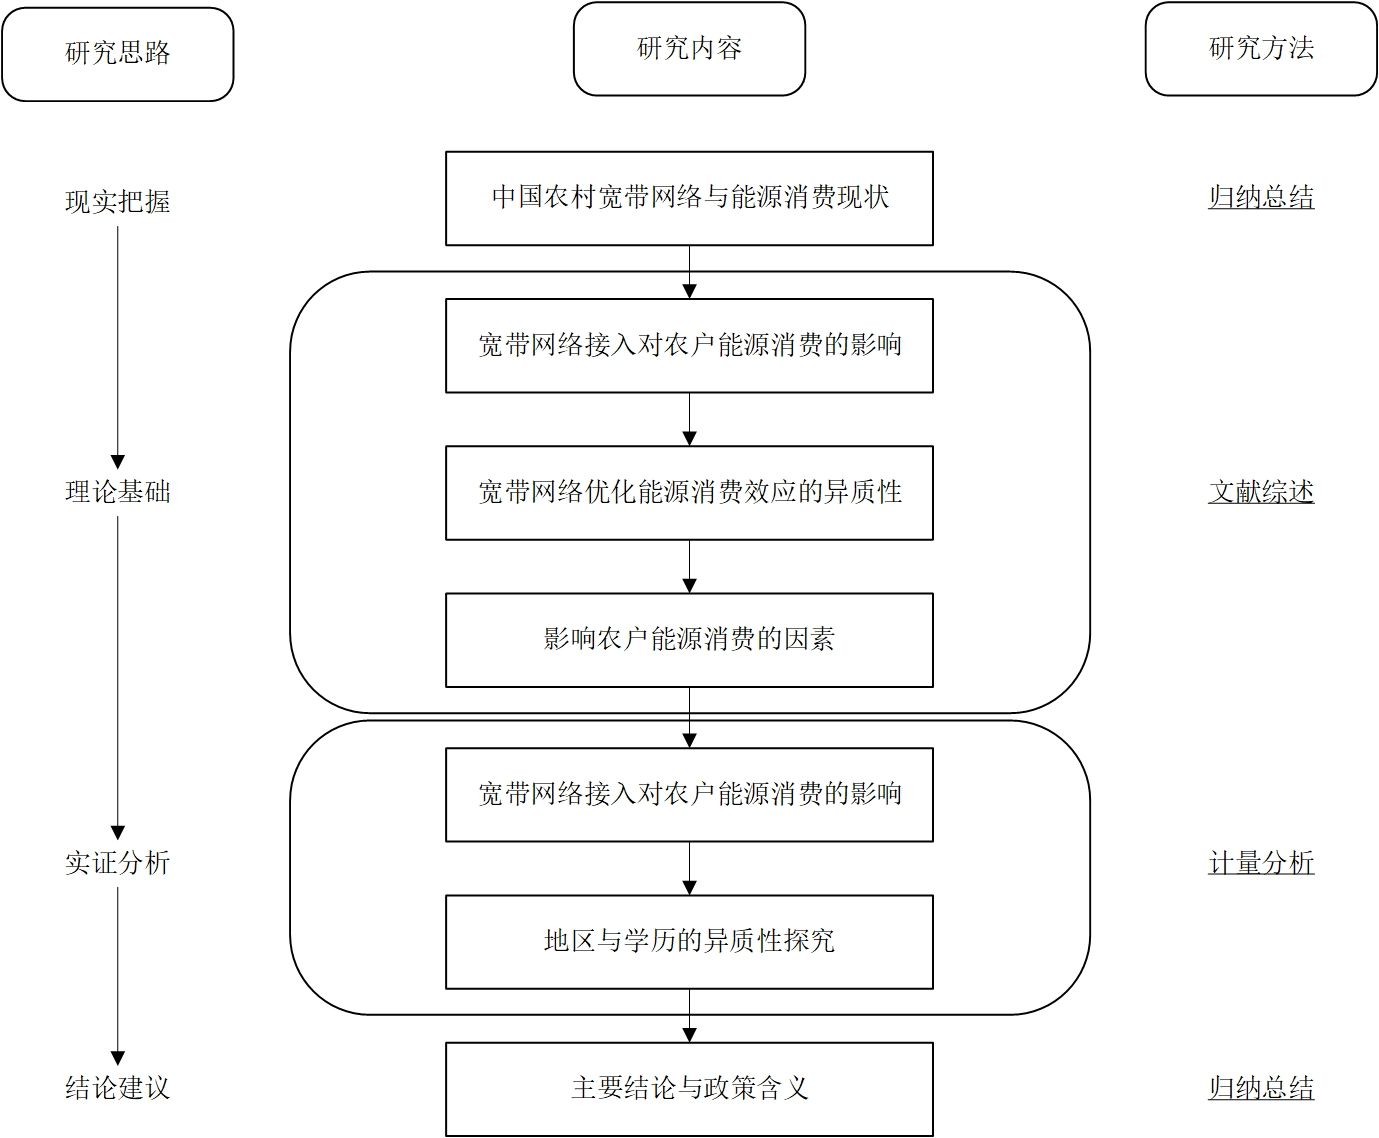
\includegraphics[width = 1\textwidth]{技术路线.jpg}
		{\heiti \zihao{-4} \caption{技术路线}}
	\end{figure*}
	\section{文献回顾与理论假说}
	\subsection{理论依据一}
	首先,宽带网络作为信息技术的进步,有利于打破农村信息困境,使农户获得能源相关的知识与能源政策的信息。由于我国的农村普遍落后于城市,在能源消费上,消费结构较为复杂,仍大量存在着使用传统能源的农户,在信息资源的获取上,时常受到约束,相比于城市居民,农户一直是信息弱势群体;农村地区信息资源匮乏,信息落后和失真现象严重,难以接收到能源相关的知识与信息,通过接入宽带,有利于改变农村地区信息获取难的困境(姜维军等,2021)。在过去,政府通常是农户获取信息的重要途径(Knight et al, 2015),由于经过重重审核,政府所提供的信息量较少且时效性较差,难以满足农户日益增长的信息需求(De Groot et al,2001)。但随着我国农村互联网基础设施的不断完善,农户可以通过电脑、手机等设备获取信息,降低了信息获取的成本(李文欢和王桂霞,2021),打破了信息资源的约束(李文欢和王桂霞,2021;闫贝贝等,2020),但对于不同的上网群体,仍旧存在较大的“数字鸿沟”,进而导致互联网信息并没有对所有农户的能源消费行为产生相应的影响,有学者对数字鸿沟进行过解释,认为信息的可接入性是“一级数字鸿沟”(许竹青等,2013),主要囊括了上网设备的获取难度以及宽带网络的覆盖广度等,信息的利用与鉴别是“二级数字鸿沟”(许竹青等,2013),主要是指网络使用者是否通过网络获取了能源消费相关的信息,并将信息转化为对能源的认知,即信息检索与信息处理的能力。即使互联网媒体对能源政策、能源问题进行过大量报道,政府对农村地区能源升级出台优惠性政策,由于“数字鸿沟”的存在,农户也难以接收到准确且具备时效性的信息,因此宽带网络接入首先能够降低农户处于信息弱势的地位,进而利用互联网信息做出能源消费抉择。为了实证分析宽带网络接入对农户能源消费的影响,本文提出研究假说一:
	
	~\
	\begin{figure}[htbp]
		\centering
		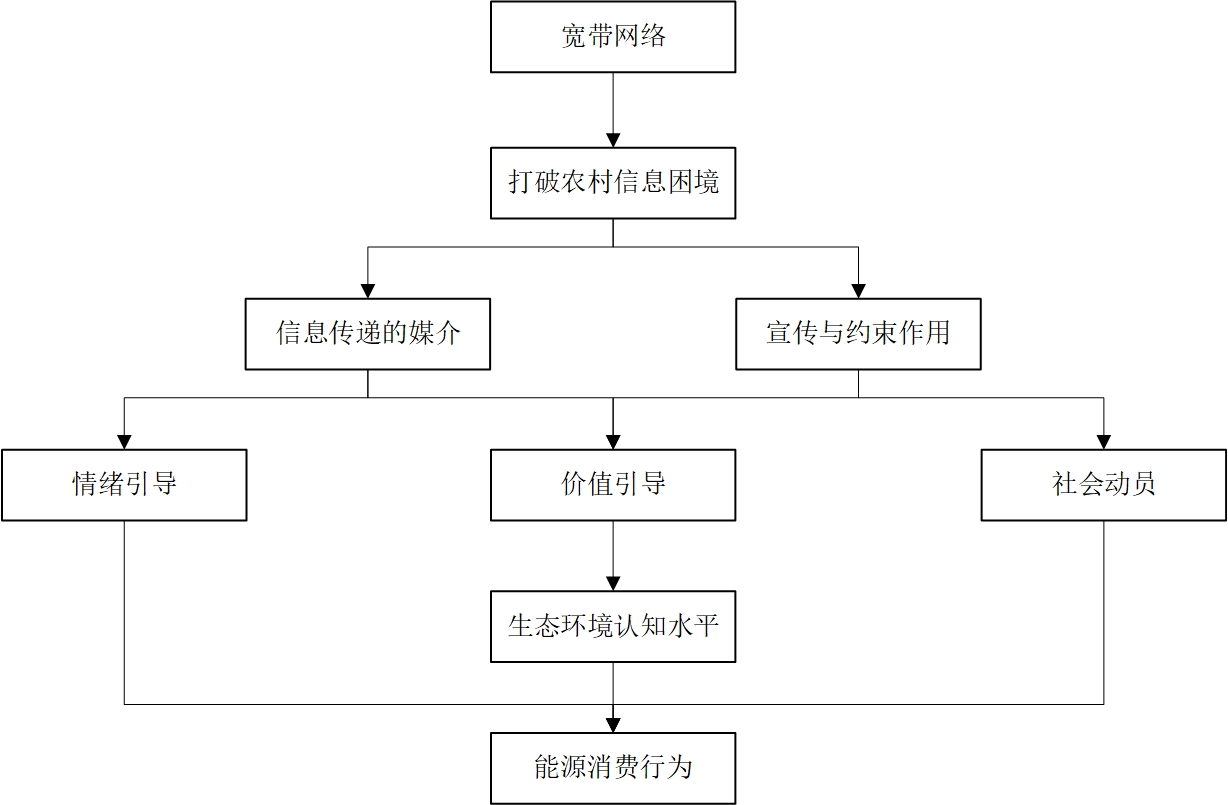
\includegraphics[width = 1\textwidth]{影响机制.jpg}
		{\heiti \zihao{-4} \caption{影响机制}}
	\end{figure}
	\subsection{理论依据二}
	\subsection{理论依据三}
	\subsection{文献述评}
	\section{数据来源与统计学特征}
	\subsection{数据来源}
	\subsection{统计学特征}
	\section{变量选取与模型设定}
	\subsection{变量选取}
	\subsubsection{被解释变量}
	有相关研究表明,更好的清洁性、便利性、高效性一般在“能源阶梯理论”中较高层级的能源中才能体现(Van et al,2008),收入高的群体在选择能源时往往更注重卫生性、便利性、舒适性(陆慧和卢黎,2006),魏楚和韩晓则依据能源的便利性、清洁性、高效性,将能源分为三类,即生物质能(不具备三性)、只占有其中两性的低劣能源以及三性兼备的商品能源(魏楚和韩晓,2018),因此本文依据能源的属性对问卷中涉及的具体能源进行归类,详情见\ref{表1},最终划分得到三个二值变量:是否使用生物质能(bio)、是否使用低劣能源(trad)、是否使用商品能源(modern),分别作为三个基准回归模型的被解释变量。
	
	~\
	\begin{table}[htbp]
		\centering
		{\heiti \zihao{-4} \caption{概念定义:能源构成}}
		\label{表1}
		\begin{tabular}{llllll}
			\cline{1-3}
			\multicolumn{1}{c}{\textbf{能源大类}}         & \multicolumn{1}{c}{\textbf{能源小类}} & \multicolumn{1}{c}{\textbf{组成部分}}          &  &  &  \\ \cline{1-3}
			\multicolumn{1}{c}{\multirow{2}{*}{传统能源}} & \multicolumn{1}{c}{生物质能}          & \multicolumn{1}{c}{禽畜粪便、农作物秸秆、薪柴}          &  &  &  \\
			\multicolumn{1}{c}{}                      & \multicolumn{1}{c}{低劣能源}          & \multicolumn{1}{c}{蜂窝煤、煤球、煤块}              &  &  &  \\
			\multicolumn{1}{c}{现代能源}                  & \multicolumn{1}{c}{商品能源}          & \multicolumn{1}{c}{瓶装液化气、汽油、柴油、管道煤气、管道天然气} &  &  &  \\ \cline{1-3}
		\end{tabular}
	\end{table}
	\subsubsection{解释变量}
	\subsection{模型设定}
	首先,考虑使两点的分布介于0到1之间,在给定$x$的情况下,$y$的两点分布概率如下:
	\begin{equation}
		\left\{ \begin{array}{l}
			P(y=1\mid x)=F(x,\beta )\\
			P(y=0\mid x)=1-F(x,\beta )\\
		\end{array} \right. 
	\end{equation}
	若$F(x,\beta )$为服从Logistic分布的累积分布函数时,Logistic函数表达式如下:
	\begin{equation}
		\mathrm{P(}y=1\mid x)=F(x,\beta )=\Lambda \left( x^{'}\boldsymbol{\beta } \right) \equiv \frac{\exp \left( x^{'}\boldsymbol{\beta } \right)}{1+\exp \left( x^{'}\boldsymbol{\beta } \right)}
	\end{equation}
	其中$\left( x'\beta \right)$构成线性组合,具体形式如下:
	\begin{equation}
		x'\beta =\beta _0+\beta _1x_1+\beta _2x_2+\cdots +\beta _ix_i=\beta _0+\sum_{i=1}^i{\beta _i}x_i
	\end{equation}
	$i$代表研究中所涉及的不同解释变量。
	
	为方便对Logistic模型的结果进行解释,将(2)进行参数的线性变换后得到最终形式,称为Logit模型:
	\begin{equation}
		\ln \left( \frac{P}{1-P} \right) =x^{'}\beta
	\end{equation}
	Logit模型为本文的基准回归模型。
	
	若$F(x,\beta )$为标准正态分布的累积分布函数,则:
	\begin{equation}
		\mathrm{P(}y=1\mid x)=F(x,\beta )=\Phi \left( x^{'}\beta \right) \equiv \int_{-\infty}^{x^{'}\beta}{\phi}(t)\mathrm{d}t
	\end{equation}
	模型(5)称为Probit模型, $\phi (t)$为标准正态分布的概率密度函数,本文将使用Probit模型进行基准回归模型的稳健性检验分析。
	\section{计量结果与实证分析}
	
	\subsection{基准回归模型}
	
	\subsubsection{模型一的结果}
	
	\subsubsection{模型二的结果}
	
	\subsubsection{模型三的结果}
	
	\subsection{稳健性检验}
	
	\subsubsection{检验方式一}
	
	\subsubsection{检验方式二}
	
	\subsubsection{检验方式三}
	
	\subsection{异质性分析}
	
	\subsubsection{异质性一}
	
	\subsubsection{异质性二}
	
	\section{拓展性探究}
	
	\section{主要结论与政策含义}
	
	\newpage
	\section*{\centerline{参 \enspace 考 \enspace 文 \enspace 献}}
	\addcontentsline{toc}{section}{参考文献}
	\vspace{-8mm}
	{\setlength{\parindent}{0pt}
	姜维军, 颜廷武, 张俊飚. 互联网使用能否促进农户主动采纳秸秆还田技术——基于内生转换Probit 模型的实证分析[J]. 农业技术经济, 2021(03): 50-62.
	
	廖华. 中国农村居民生活用能现状、问题与应对[J]. 北京理工大学学报(社会科学版), 2019, 21(02): 1-5.
	
	李文欢, 王桂霞. 互联网使用有助于农户参与黑土地质量保护吗?[J]. 干旱区资源与环境, 2021, 35(07): 27-34.
	
	陆慧, 卢黎. 农民收入水平对农村家庭能源消费结构影响的实证分析[J]. 财贸研究, 2006(03): 28-34.
	
	苏芳, 梁秀芳, 尚海洋等. 收入多样性对农户能源消费结构的影响——以陕南秦巴山区为例[J]. 资源开发与市场, 2022, 38(01): 78-85.
	
	魏楚, 王丹, 吴宛忆等. 中国农村居民煤炭消费及影响因素研究[J]. 中国人口·资源与环境, 2017, 27(09): 178-185.
	
	许竹青,郑风田,陈洁.“数字鸿沟”还是“信息红利”?信息的有效供给与农民的销售价格——一个微观角度的实证研究[J].经济学(季刊),2013,12(04):1513-1536
	
	闫贝贝, 张强强, 刘天军. 手机使用能促进农户采用IPM技术吗[J]. 农业技术经济, 2020(05): 45-59.
	
	郑新业. 中国家庭能源消费研究报告[M]. 中国家庭能源消费研究报告, 2016.
	
	De Groot H L, Nijkamp P, Acs Z. Knowledge spill-overs, innovation and regional development: Springer, 2001: 249-253.
	
	Knight D W, Allegretti A M, Vaske J J. Information dissemination-diffusion and marine protected area approval in the Philippines[J]. Ocean \& Coastal Management, 2015, 113: 38-46.

	Van Ruijven B, Urban F, Benders R M, et al. Modeling energy and development: an evaluation of models and concepts[J]. World Development, 2008, 36(12): 2801-2821.}

	% --------------------附录--------------------
	\newpage
	\section*{附录A:图表}
	\addcontentsline{toc}{section}{附录A:图表}
	\vspace{-8mm}
	
	\newpage
	\section*{附录B:计算程序}
	\addcontentsline{toc}{section}{附录B:计算程序}
	\vspace{-8mm}
	
	\newpage
	\section*{\centerline{致 \qquad 谢}}
	\addcontentsline{toc}{section}{致谢}
	\vspace{-8mm}

\end{document}